\documentclass[11pt,class=report,crop=false]{standalone}
\usepackage[screen]{../python}


\begin{document}


%====================================================================
\chapitre{Fonctions de plusieurs variables}
%====================================================================

\insertvideo{twrd6e89vaA}{partie 3.1. Définition et graphe}

\insertvideo{sCjEukXJoGw}{partie 3.2. Minimums et maximums}

\insertvideo{txGgbSganSA}{partie 3.3. Recherche d'un minimum}



\objectifs{Dans ce chapitre, nous allons nous concentrer sur les fonctions de deux variables et la visualisation de leur graphe et de leurs lignes de niveau. 
La compréhension géométrique des fonctions de deux variables est fondamentale pour assimiler les techniques qui seront rencontrées plus tard avec un plus grand nombre de variables.}


De nombreux phénomènes dépendent de plusieurs paramètres, par exemple le volume d'un gaz dépend de la température et de la pression; l'altitude $z$ d'un terrain dépend des coordonnées $(x,y)$ du lieu.

Dans les réseaux de neurones, les fonctions de plusieurs variables interviennent de deux manières :
\begin{itemize}
  \item lors de l'utilisation d'un réseau. C'est la partie la plus facile et la plus fréquente. On utilise un réseau déjà bien paramétré pour répondre à une question (Est-ce une photo de chat ? Tourner à droite ou à gauche ? Quel pion déplacer au prochain coup ?). La réponse est un calcul direct obtenu en évaluant une fonction de plusieurs variables. 
  
  \item lors de la paramétrisation du réseau. C'est la partie difficile et le but de ce cours. Quels paramètres choisir pour définir ce réseau afin qu'il réponde au problème ? Ces paramètres seront choisis comme minimum d'une fonction de plusieurs variables. Une des difficultés est qu'il peut y avoir des milliers de paramètres à gérer.
  
\end{itemize}




%%%%%%%%%%%%%%%%%%%%%%%%%%%%%%%%%%%%%%%%%%%%%%%%%%%%%%%%%%%%%%%%%%%%%
\section{Définition et exemples}

%--------------------------------------------------------------------
\subsection{Définition}


Nous allons étudier les fonctions de deux variables, mais aussi de trois variables et plus généralement de $n$ variables.
Ces fonctions sont donc de la forme 
$$f : \Rr^n \rightarrow \Rr$$
où $n$ est un entier naturel supérieur ou égal à $1$. 


Un élément de l'ensemble de départ est un vecteur de type  $x = (x_1,\ldots,x_n)$. À chacun de ces vecteurs, $f$ associe un nombre réel $f(x_1,\ldots,x_n)$. On pourrait aussi limiter l'ensemble de départ à une partie $E$ de $ \Rr^n$.



%--------------------------------------------------------------------
\subsection{Deux variables}

Lorsque $n=2$, on préfère noter les variables $(x,y)$ plutôt que $(x_1,x_2)$.
Voici quelques exemples.
\begin{exemple}
\sauteligne
\begin{itemize}
  \item $f(x,y) = 2x+3y^2+1$.
  \item $f(x,y) = \cos(xy)$.
  \item $f(x,y) = \sqrt{x^2+y^2}$. $f$ renvoie la distance entre un point $M(x,y)$ et l'origine $O(0,0)$.
  
   \myfigure{1}{
     \tikzinput{fig-fonctions-01}
   }
  
  \item L'équation physique $PV=nRT$ implique $T = \frac{1}{nR}PV$ :
  la température d'un gaz s'exprime en fonction de son volume et de la pression ($n$ et $R$ sont des constantes).
  \item La distance entre une droite fixée $\mathcal{D}$ d'équation $ax+by+c=0$ et un point $M(x_0,y_0)$ est donnée par une fonction de deux variables : $$d(x_0,y_0) = d(M,\mathcal{D}) = \frac{|ax_0+by_0+c|}{\sqrt{a^2+b^2}}.$$

   \myfigure{1}{
     \tikzinput{fig-fonctions-02}
   }
  
  
\end{itemize}
\end{exemple}


%--------------------------------------------------------------------
\subsection{Trois variables}

\begin{exemple}
\sauteligne
\begin{enumerate}
  \item $f(x,y,z) = ax+by+cz+d$. Cette fonction $f$ est une fonction affine ($a,b,c,d$ sont des constantes).
   \item $f(x,y,z) = x^2+y^2+z^2$ qui donne la distance au carré entre un point $M(x,y,z)$ et l'origine $O(0,0,0)$.
   \item Le volume d'un cône à base rectangulaire dépend des longueurs des côtés $a$ et $b$ de la base et de la hauteur $h$ :
   $$V = f(a,b,h) = \frac13 abh.$$
   
   \myfigure{0.5}{
     \tikzinput{fig-fonctions-03}
   }
     
\end{enumerate}
\end{exemple}


%--------------------------------------------------------------------
\subsection{$n$ variables}

\begin{exemple}
\sauteligne
\begin{enumerate}
  \item $f(x_1,\ldots,x_n) = a_1x_1+\cdots+a_nx_n+a_0$ une fonction affine (les $a_i$ sont des constantes).
  \item $f(x_1,\ldots,x_n) = \sqrt{(x_1-a_1)^2+\cdots+(x_n-a_n)^2}$ exprime la distance entre les points $M(x_1,\ldots,x_n)$ et $A(a_1,\ldots,a_n)$ dans $\Rr^n$.
\end{enumerate}
\end{exemple}


%%%%%%%%%%%%%%%%%%%%%%%%%%%%%%%%%%%%%%%%%%%%%%%%%%%%%%%%%%%%%%%%%%%%%
\section{Graphe}

Le cas le plus simple, et déjà connu, est celui des fonctions d'une seule variable $f : \Rr \rightarrow \Rr$.  C'est l'ensemble de tous les points du plan de la forme $(x,f(x))$. Voici le graphe de la fonction $x \mapsto x\cos x$.

\myfigure{0.8}{
  \tikzinput{fig-fonctions-04}
} 



%--------------------------------------------------------------------
\subsection{Définition}





\begin{definition}
Le \defi{graphe} $\mathcal{G}_f$ d'une fonction de deux variables $f : \Rr^2 \to \Rr$ est  l'ensemble des points de $\Rr^3$ ayant pour coordonnées $(x,y,f(x,y))$, pour $(x,y)$ parcourant $\Rr^2$. Le graphe est donc :
$$\mathcal{G}_f= \big\{ (x,y,z) \in \Rr^3 \mid (x,y)\in \Rr^2 \text{ et } z=f(x,y)\big\}.$$
\end{definition}

Dans le cas de deux variables, le graphe d'une fonction est une surface tracée dans l'espace.


   \myfigure{0.7}{
     \tikzinput{fig-fonctions-05}
   }
   

\begin{exemple}
On souhaite tracer le graphe de la fonction définie par :
$$f(x,y) = x  e^{-x^2-y^2}.$$

On commence par tracer quelques points à la main :
\begin{itemize}
  \item si $(x,y) = (0,0)$ alors $f(x,y) = f(0,0) = 0$ donc le point de coordonnées $(0,0,0)$ appartient au graphe.
  \item Comme $f(1,0) = 1/e$ alors le point de coordonnées $(1,0,1/e)$ appartient au graphe.
  \item Pour n'importe quel $y$, on a $f(0,y)=0$ donc la droite de l'espace d'équation ($x=0$ et $z=0$) est incluse dans le graphe.
  \item Notons $r = \sqrt{x^2+y^2}$ la distance entre le point de coordonnées $(x,y)$ et l'origine $(0,0)$ alors on a la formule $f(x,y) = x e^{-r^2}$. Pour un point éloigné de l'origine, $r$ est grand, donc  $e^{-r^2}$ est très petit, et $f(x,y)$ est très proche de $0$.
\end{itemize}


Voici différentes vues de ce graphe.

\begin{center}
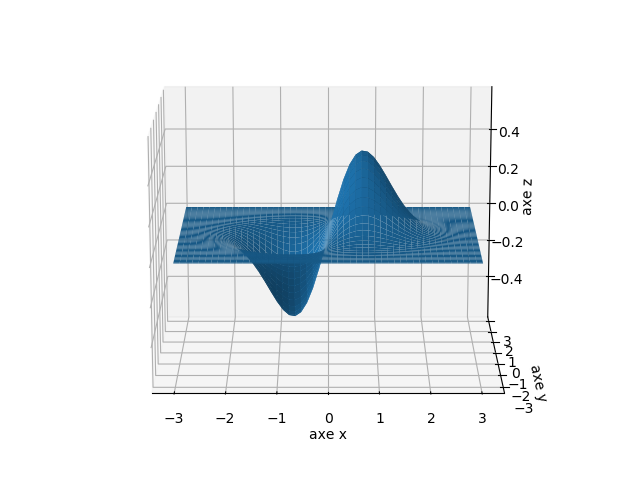
\includegraphics[scale=\myscale,scale=0.5]{figures/fonctions-surface-1a}
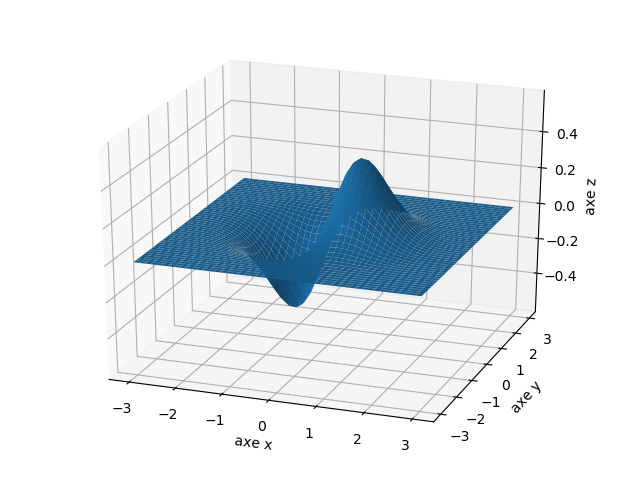
\includegraphics[scale=\myscale,scale=0.5]{figures/fonctions-surface-1b}
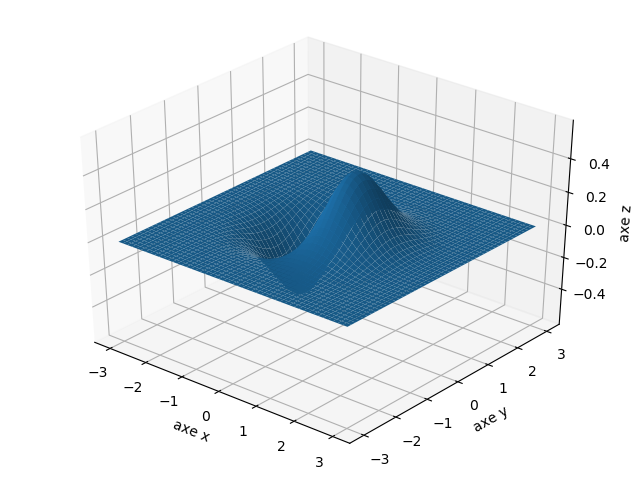
\includegraphics[scale=\myscale,scale=0.5]{figures/fonctions-surface-1c}
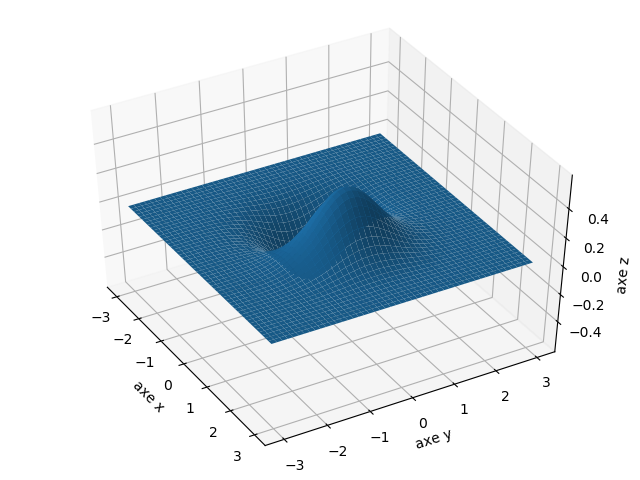
\includegraphics[scale=\myscale,scale=0.5]{figures/fonctions-surface-1d}
\end{center}

%  fichier python 'fonctions-surface-1.py'
\end{exemple}


%--------------------------------------------------------------------
\subsection{Tranches}

Afin de tracer le graphe d'une fonction de deux variables, on peut découper la surface en \og{}tranches\fg{}.
On fixe par exemple une valeur $y_0$ et on trace dans le plan $(xOz)$ le graphe de la fonction d'une variable  
$$f_{|y_0} : x\mapsto f(x,y_0).$$
Géométriquement, cela revient à tracer l'intersection du graphe de $f$ et du plan d'équation $(y=y_0)$.
On recommence pour plusieurs valeurs de $y_0$, ce qui nous donne des tranches du graphe de $f$ et nous donne une bonne idée du graphe complet de $f$.

On peut faire le même travail en fixant des valeurs $x_0$ avec les fonctions :
$$f_{|x_0} : y \mapsto f(x_0,y).$$


\begin{exemple}
On souhaite tracer le graphe de la fonction définie par :
$$f(x,y) = x \sin(y).$$

\begin{center}
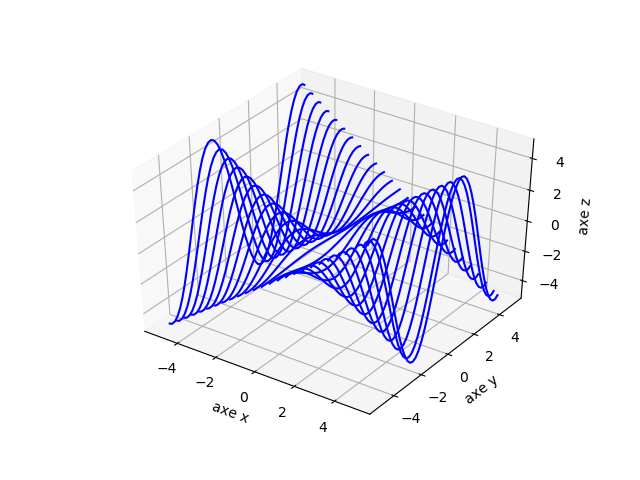
\includegraphics[scale=\myscale,scale=0.5]{figures/fonctions-surface-2a}
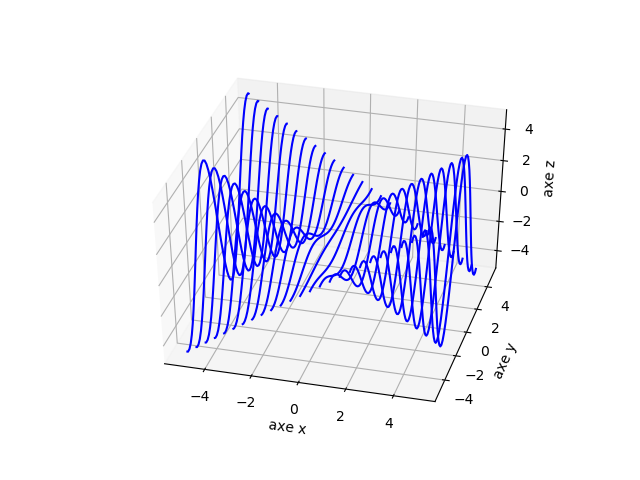
\includegraphics[scale=\myscale,scale=0.5]{figures/fonctions-surface-2b}
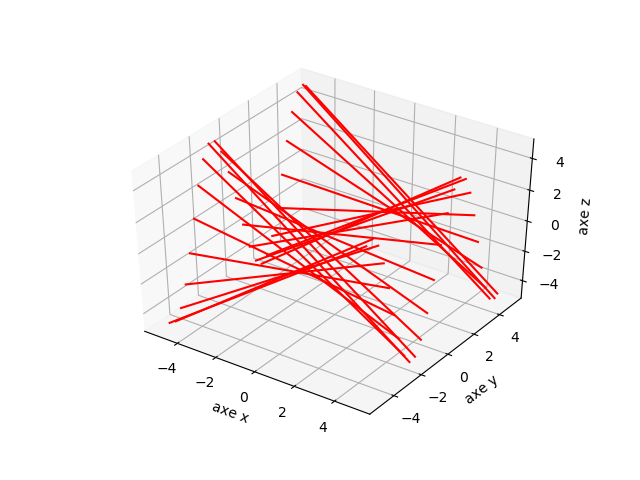
\includegraphics[scale=\myscale,scale=0.5]{figures/fonctions-surface-2c}
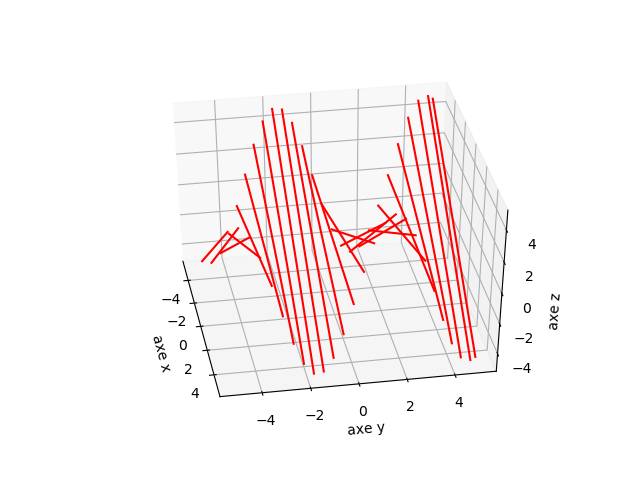
\includegraphics[scale=\myscale,scale=0.5]{figures/fonctions-surface-2d}

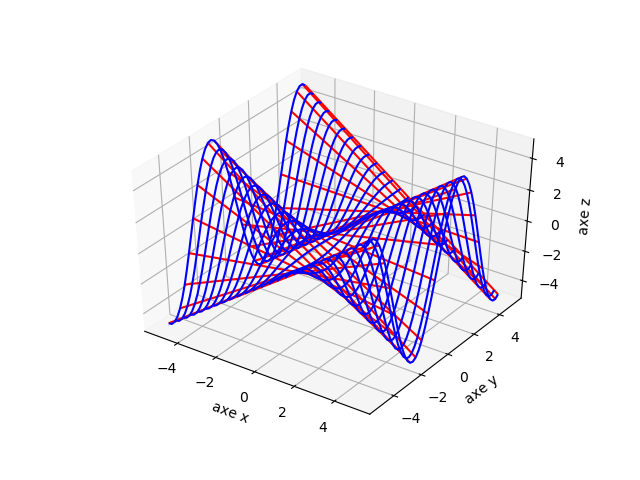
\includegraphics[scale=\myscale,scale=0.7]{figures/fonctions-surface-2e}
\end{center}

\couleurnb{En bleu}{En haut} les tranches pour lesquelles $x$ est constant (deux points de vue), \couleurnb{en rouge}{au milieu} les tranches pour lesquelles $y$ est constant (deux points de vue). Lorsque l'on rassemble les tranches (à $x$ constant et à $y$ constant), on reconstitue la surface (dernière figure). 

% voir fichier python 'fonctions-surface-2.py'

\end{exemple}


%--------------------------------------------------------------------
\subsection{Minimum, maximum}

Pour des fonctions de deux variables (ou plus) il existe une notion de minimum et de maximum.


\begin{definition}
\index{minimum!local}
\index{minimum!global}
Soit $f : \Rr^2 \to \Rr$ une fonction.
\begin{itemize}
  \item $f$ atteint un \defi{minimum global} en $(x_0,y_0) \in \Rr^2$ si
  pour tout $(x,y) \in \Rr^2$, on a $f(x,y) \ge f(x_0,y_0)$.
  
  \item $f$ atteint un \defi{minimum local} en $(x_0,y_0) \in \Rr^2$ si
  il existe un intervalle ouvert $I$ contenant $x_0$ et un intervalle ouvert $J$ contenant $y_0$  tels que 
  pour tout $(x,y) \in I \times J$, on a $f(x,y) \ge f(x_0,y_0)$. 
\end{itemize}
\end{definition}



\begin{exemple}
Voici l'exemple d'une fonction qui admet deux minimums locaux. L'un est aussi un minimum global. Elle admet un maximum local qui est aussi global.

\begin{center}
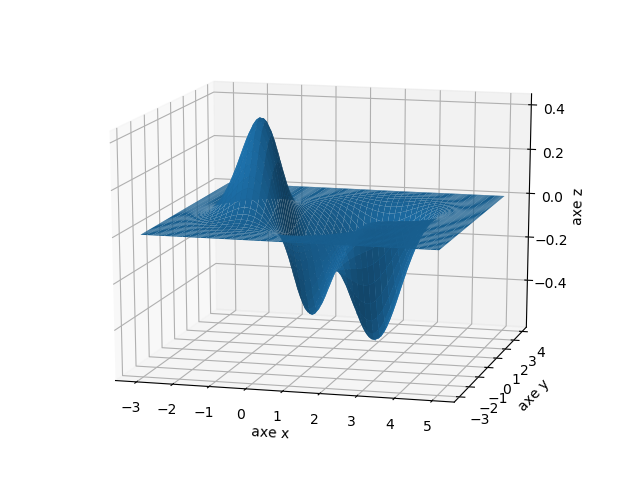
\includegraphics[scale=\myscale,scale=0.7]{figures/fonctions-surface-3}
\end{center}

% voir fichier python 'fonctions-surface-3.py'

\end{exemple}


Trouver les bons paramètres d'un réseau de neurones nous amènera à trouver le minimum d'une fonction de plusieurs (et même de centaines de) variables. Voyons un exemple en deux variables.
\begin{exemple}
Étant donnés trois points $A(1,2)$, $B(3,5)$ et $C(6,1)$, il s'agit de trouver un point $M(x,y)$ qui \og{}approche au mieux\fg{} ces trois points. Il faut expliciter une fonction à minimiser pour définir correctement le problème. Nous décidons de prendre la somme des carrés des distances.


   \myfigure{1}{
     \tikzinput{fig-fonctions-06}
   }
   
Il s'agit donc de minimiser la fonction $f$ suivante, qui correspond à une fonction distance (aussi appelée fonction erreur ou bien fonction coût) :
$$f(x,y) = MA^2+MB^2+MC^2 = 
(x-1)^2+ (y-2)^2 + (x-3)^2 + (y-5)^2 + (x-6)^2 + (y-1)^2.$$
En développant on trouve :
$$f(x,y) = 3x^2 + 3y^2 - 20x - 16y + 76.$$

Le graphe de $f$ nous suggère qu'il existe un unique minimum qui est le minimum global de $f$. 
 Par recherche graphique ou par les méthodes décrites dans la section suivante, on trouverait une solution approchée. En fait la solution géométrique exacte est l'isobarycentre des points (autrement dit le centre de gravité du triangle $ABC$), ainsi :
 $$(x_0,y_0) = \left(\frac{10}{3},\frac83\right) \simeq (3.33,2.66)$$
 pour lequel $f$ atteint son minimum $z_0 = f(x_0,y_0) = \frac{64}{3} \simeq 21.33$.

\begin{center}
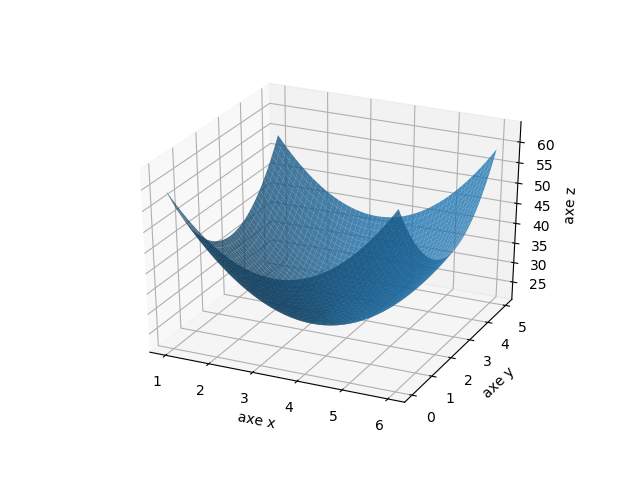
\includegraphics[scale=\myscale,scale=0.7]{figures/fonctions-surface-4}
\end{center}

% voir fichier python 'fonctions-surface-4.py'
% voir fichier sage 'fonctions-surface-4.sage' pour résolution exacte

Le point qui convient le mieux à notre problème et en lequel notre fonction distance est minimale est donc le point de coordonnées $(\frac{10}{3},\frac83)$. Attention, un autre choix de la fonction distance $f$ pourrait conduire à une autre solution (voir l'exemple de la prochaine section).

   \myfigure{1}{
     \tikzinput{fig-fonctions-07}
   }


\end{exemple}

%--------------------------------------------------------------------
\subsection{Recherche élémentaire d'un minimum}


Voici trois techniques pour trouver les valeurs approchées des coordonnées du point en lequel une fonction de plusieurs variables atteint son minimum. Ces techniques sont valables quelque soit le nombre de variables même si ici elles ne sont décrites que dans le cas de deux variables. 

\textbf{Recherche sur une grille.} On calcule $f(x,y)$ pour $(x,y)$ parcourant une grille. On retient le point $(x_0,y_0)$ en lequel $z_0=f(x_0,y_0)$ est le plus petit. Si on le souhaite, on peut affiner la grille autour de ce point, en diminuant le pas $\epsilon$ pour améliorer l'approximation. C'est une technique qui demande $N^2$ calculs pour une grille de largeur $N$ (et même $N^n$ pour une fonction de $n$ variables) ce qui peut être énorme.

   \myfigure{0.5}{
     \tikzinput{fig-fonctions-08}
   }


\textbf{Recherche au hasard.} Cela peut sembler incongru mais choisir quelques coordonnées $(x,y)$ au hasard, calculer chaque valeur $z=f(x,y)$ et comme auparavant retenir le point $(x_0,y_0)$ correspondant au $z_0$ minimal n'est pas ridicule !
Un ordinateur peut tester plusieurs millions de points en quelques secondes. Bien sûr il y a de fortes chances de ne trouver qu'une solution approchée. C'est aussi une technique que l'on retrouvera plus tard : partir d'un point au hasard pour ensuite construire une suite de points convergeant vers un minimum. Et si cela n'est pas concluant, il faudra repartir d'un autre point tiré au hasard.

\bigskip

\textbf{Recherche par tranche.} 
L'idée est de se ramener à des fonctions d'une seule variable. En effet, 
pour les fonctions d'une variable, on sait qu'il faut chercher les minimums là où la dérivée s'annule.

On part d'une valeur $x_0$ (au hasard !). On cherche le minimum sur la tranche $x=x_0$, c'est-à-dire que l'on cherche le minimum de la fonction d'une variable $y \mapsto f(x_0,y)$. On trouve une valeur $y_0$ qui réalise un minimum. On change alors de direction en étudiant maintenant la tranche $y=y_0$ (pour le $y_0$ que l'on vient d'obtenir), on obtient l'abscisse $x_1$ du minimum de la fonction d'une variable $x \mapsto f(x,y_0)$. On recommence depuis le début à partir de ce $x_1$. On obtient ainsi une suite de points $(x_i,y_i)$ avec des valeurs $z_i=f(x_i,y_i)$ de plus en plus petites. On peut espérer tendre vers un minimum. %que $(x_i,y_i)$ tendent vers un minimum.


   \myfigure{1}{
     \tikzinput{fig-fonctions-09}
   }
   
Sur la figure ci-dessus, on part d'une tranche \couleurnb{(en bleu) }{}choisie au hasard, donnée par $x=x_0$. Cette tranche définit le graphe d'une fonction d'une variable. On se déplace sur cette courbe jusqu'à atteindre le minimum de cette tranche, en une valeur $y_0$. On considère la tranche perpendiculaire donnée par $y=y_0$. On se déplace sur la courbe \couleurnb{rouge }{}jusqu'à atteindre le minimum de cette tranche, en une valeur $x_1$. On pourrait continuer avec une nouvelle tranche \couleurnb{bleue }{}$x=x_1$, etc.

\bigskip

Les descriptions données ici sont assez informelles, d'une part parce qu'il est difficile d'énoncer des théorèmes qui garantissent d'atteindre un minimum local et d'autre part parce qu'aucune technique ne garantit d'atteindre un minimum global. Lorsque l'on étudiera le gradient, nous obtiendrons une méthode plus efficace.

\begin{exemple}
On reprend le problème précédent, à savoir trouver un point $M$ qui approche au mieux les trois points $A$, $B$ et $C$, mais cette fois on choisit la \og{}vraie\fg{} distance comme fonction d'erreur :
$$g(x,y) = MA+MB+MC = 
\sqrt{(x-1)^2+ (y-2)^2} + \sqrt{(x-3)^2 + (y-5)^2} + \sqrt{(x-6)^2 + (y-1)^2}.$$
On applique ces trois techniques pour chercher le minimum de $g$ en se limitant au carré $[0,6]\times[0,6]$.

\begin{enumerate}

  \item Avec une grille $N\times N$. Par exemple pour $N=100$, on évalue $g$ en $10\,000$ points. On trouve $(x_{\min},y_{\min}) \simeq (2.91,2.97)$ pour une valeur $z_{\min} \simeq 7.84$. 
  
  \item Avec un tirage aléatoire de $1000$ points, on trouve par exemple :
  $(x_{\min},y_{\min}) \simeq (2.88,2.99)$ et $z_{\min} \simeq 7.84$. Le résultat est similaire à la méthode précédente, bien qu'on ait effectué $10$ fois moins de calculs.
  
  \item Par les tranches. On part de la tranche $(x=0)$. On pose $x_0=0$, la fonction à étudier
  est donc 
  $$g_{|x_0}(y) = \sqrt{1 + (y-2)^2} + \sqrt{9 + (y-5)^2} + \sqrt{36 + (y-1)^2}.$$
  C'est une fonction de la seule variable $y$ pour laquelle on possède des techniques efficaces de recherche de minimum.
  On trouve que le minimum de $g_{|x_0}$ est atteint en $y_0 \simeq 2.45$.
  On recommence avec cette fois la tranche $(y = y_0)$ et on cherche le minimum de la fonction $g_{|y_0}(x) = g(x,y_0)$. On trouve que cette fonction atteint son minimum en $x_1 \simeq 2.84$. 
  On recommence ce processus jusqu'à atteindre la précision souhaitée.
  Ainsi en $5$ étapes on obtient une valeur approchée assez précise du minimum 
  $(x_{\min},y_{\min}) \simeq (2.90579,2.98464)$ et $z_{\min} \simeq 7.83867$.
  
  
\end{enumerate}
\end{exemple}

La première conclusion à tirer de ce qui précède est que pour résoudre un problème il faut définir correctement une fonction d'erreur, c'est-à-dire celle que l'on cherche à minimiser. La solution trouvée dépend de cette fonction d'erreur choisie. 
Enfin, la méthode des tranches est une méthode efficace pour trouver un minimum d'une fonction, mais nous en découvrirons une encore meilleure en utilisant le gradient.


%%%%%%%%%%%%%%%%%%%%%%%%%%%%%%%%%%%%%%%%%%%%%%%%%%%%%%%%%%%%%%%%%%%%%
\section{Lignes de niveau}

\index{lignes de niveau}

%--------------------------------------------------------------------
\subsection{Définition}

\begin{definition}
Soit $f : \Rr^2 \to \Rr$ une fonction de deux variables. 
La \defi{ligne de niveau} $z=c\in \Rr$ est l'ensemble de tous les points $(x,y)$ vérifiant $f(x,y)=c$ :
$$L_c =\big\{(x,y)\in \Rr^2 \mid f(x,y)=c \big\}.$$
\end{definition}

La ligne de niveau $c$ est une courbe du plan $\Rr^2$. 

On peut aussi définir une \defi{courbe de niveau}, c'est l'ensemble des points de l'espace obtenus comme intersection du graphe $\mathcal{G}_f$ et du plan $z=c$ qui est horizontal et \og{}d'altitude\fg{} $c$. Ce sont donc tous les points $(x,y,f(x,y))$ avec $f(x,y)=c$. On obtient la courbe de niveau en translatant la ligne de niveau d'une altitude $c$.



\begin{exemple}
Soit $f : \Rr^2 \to \Rr$ définie par $f(x,y)=x^2+y^2$. 

  \begin{itemize}
    \item Si $c<0$, la ligne de niveau $L_c$ est vide (aucun point n'est d'altitude négative).
    \item Si $c=0$, la ligne de niveau $L_0$ se réduit à $\{(0,0)\}$.
    \item Si $c>0$, la ligne de niveau $L_c$  est le cercle du plan de centre $(0,0)$ et de rayon $\sqrt{c}$. On \og{}remonte\fg{} $L_c$ à l'altitude $z=c$ : la courbe de niveau est alors le cercle horizontal de l'espace de centre $(0,0,c)$ et de rayon $\sqrt{c}$. 
  \end{itemize}
      
Le graphe est alors une superposition de cercles horizontaux de l'espace de centre $(0,0,c)$ et de rayon $\sqrt{c}$, $c>0$.     

Ci-dessous : (a) la surface, (b) $5$ courbes de niveau, (c) $10$ courbes de niveau, (d) les lignes de niveau dans le plan.
\begin{center}
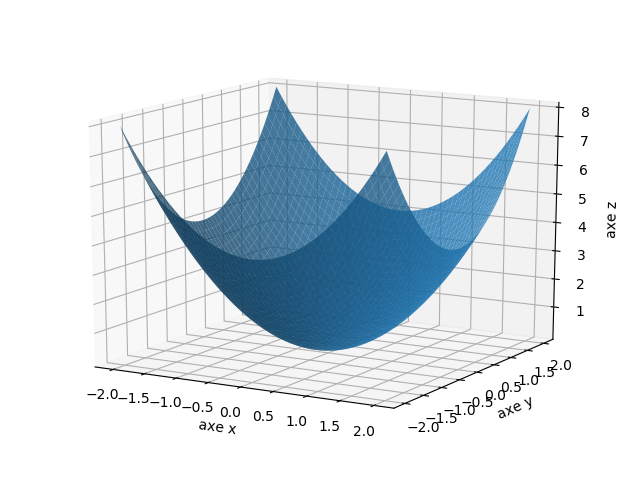
\includegraphics[scale=\myscale,scale=0.5]{figures/fonctions-niveau-1a}
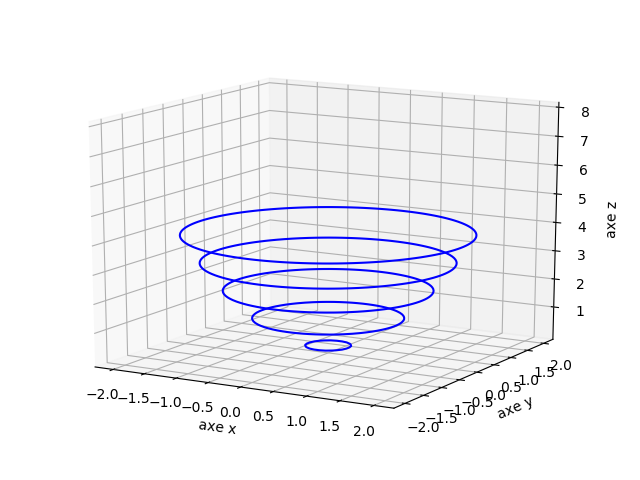
\includegraphics[scale=\myscale,scale=0.5]{figures/fonctions-niveau-1b}
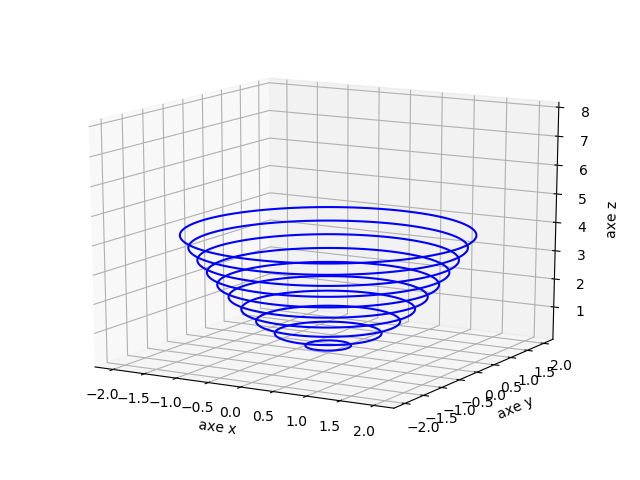
\includegraphics[scale=\myscale,scale=0.5]{figures/fonctions-niveau-1c}
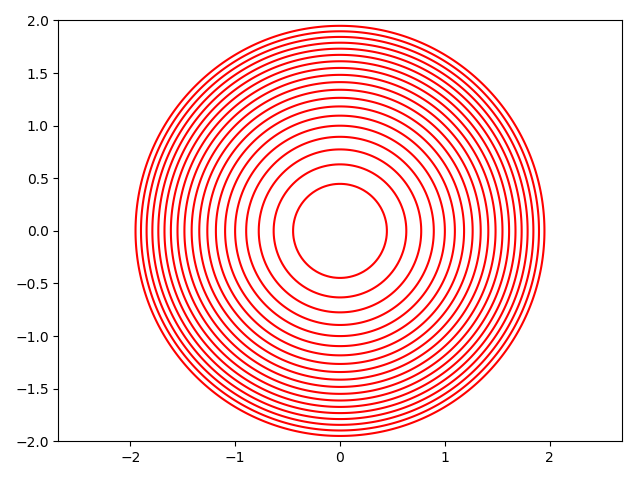
\includegraphics[scale=\myscale,scale=0.5]{figures/fonctions-niveau-1d}
\end{center}

% dessins 3d voir 'fonctions-niveau-1.py'

\end{exemple}


%--------------------------------------------------------------------
\subsection{Exemples}

\begin{exemple}
Sur une carte topographique, les lignes de niveau représentent les courbes ayant la même altitude. 
\begin{center}
  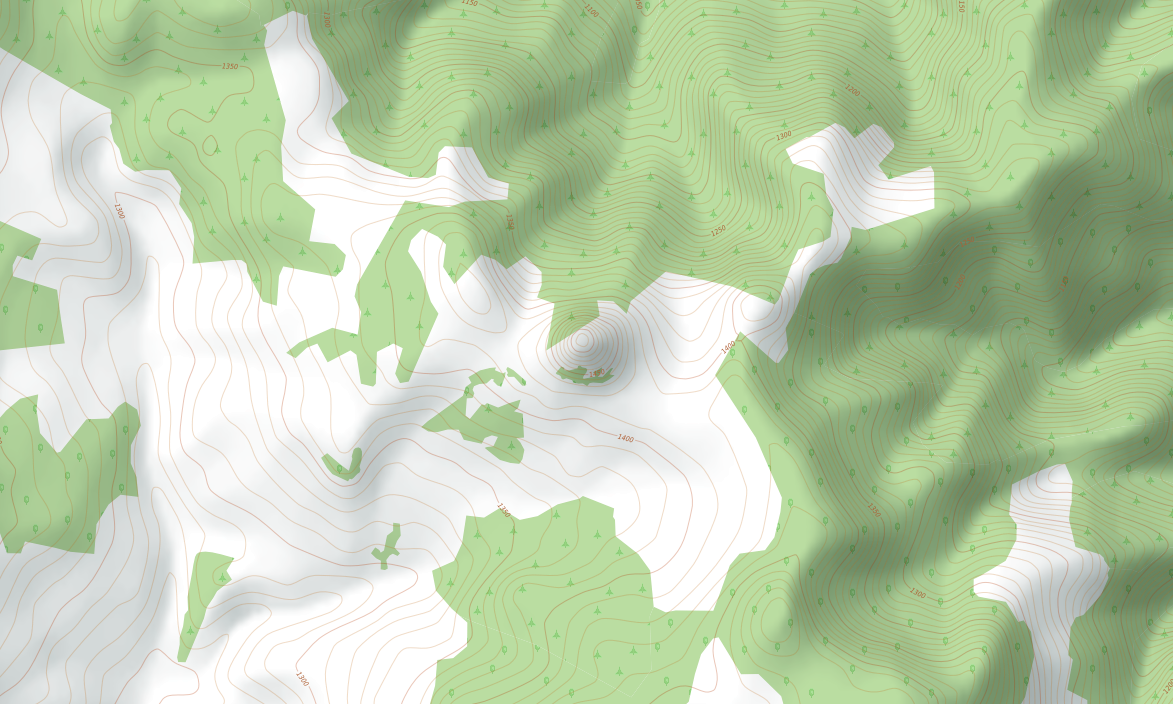
\includegraphics[scale=0.3]{figures/fig-fonctions-topo}
\end{center}
\begin{itemize}
  \item Ici, une carte \emph{Open Street Map} avec au centre le mont Gerbier de Jonc (source de la Loire, 1551 m). 
  \item Les lignes de niveau correspondent à des altitudes équidistantes de $10$ m (par exemple, pour $c=1400$, $c=1410$, $c=1420$\ldots).
  \item Lorsque les lignes de niveau sont très espacées, le terrain est plutôt plat ; lorsque les lignes sont rapprochées le terrain est pentu.
  \item Par définition, si on se promène en suivant une ligne de niveau, on reste toujours à la même altitude !
\end{itemize}
\end{exemple}



\begin{exemple}
Voici le graphe et les lignes de niveau de la fonction $f : \Rr^2 \to \Rr$ définie par
$$f(x,y) = \frac{\sin(r^2-x)}{r}+1 \quad \text{ où } r = \sqrt{x^2+y^2}.$$

\begin{center}
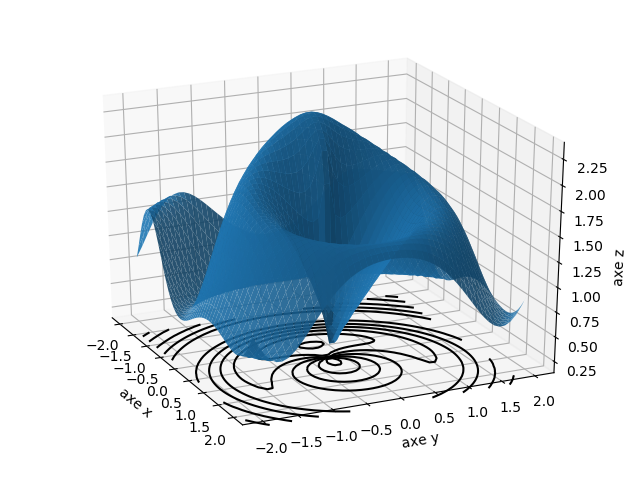
\includegraphics[scale=\myscale,scale=0.5]{figures/fonctions-niveau-2a}
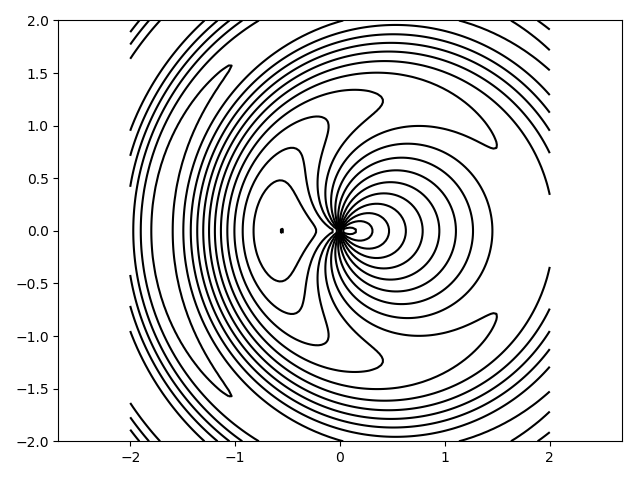
\includegraphics[scale=\myscale,scale=0.5]{figures/fonctions-niveau-2b}
\end{center}
% voir 'fonctions-niveau-2.py'


\end{exemple} 


%--------------------------------------------------------------------
\subsection{Surfaces quadratiques}

Ce sont des exemples à bien comprendre car ils seront importants pour la suite du cours.

\begin{exemple}
$$f(x,y) = \frac{x^2}{a^2} + \frac{y^2}{b^2}-1$$



\begin{itemize}
  \item Les tranches sont des paraboles.
  \item Les lignes de niveau sont des ellipses.
  \item Le graphe est donc un \defi{paraboloïde elliptique}.
\end{itemize}

Ci-dessous : (a) la surface, (b) les tranches avec $x$ constant, (c) les tranches avec $y$ constant, (d) les courbes de niveau, (e) les lignes de niveau dans le plan.

\begin{center}
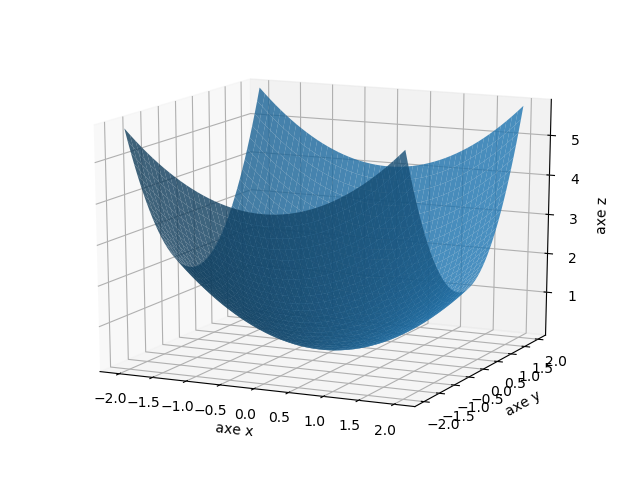
\includegraphics[scale=\myscale,scale=0.5]{figures/fonctions-quadra-1a}
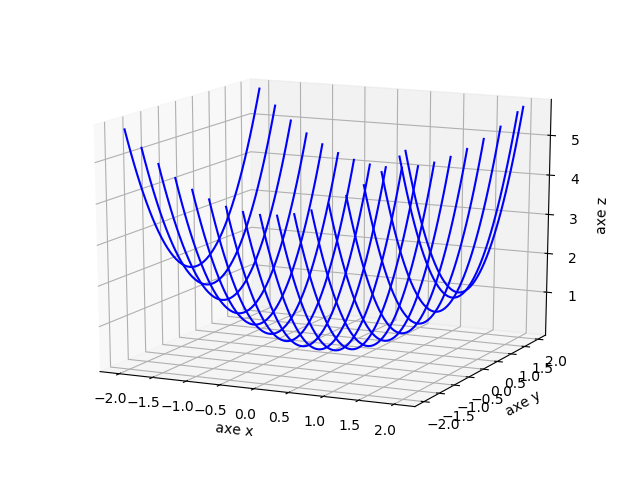
\includegraphics[scale=\myscale,scale=0.5]{figures/fonctions-quadra-1b}
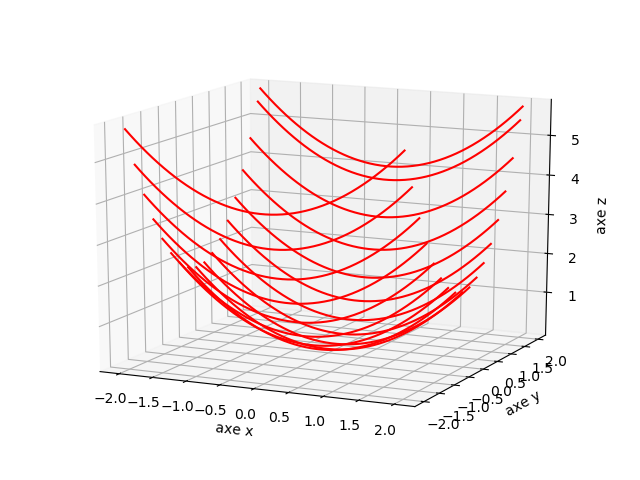
\includegraphics[scale=\myscale,scale=0.5]{figures/fonctions-quadra-1c}
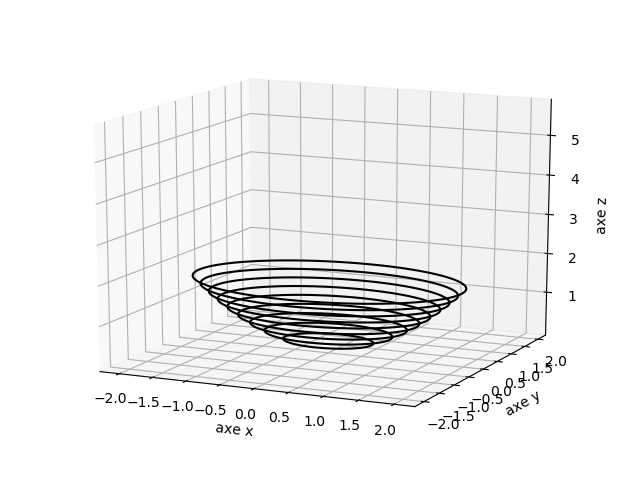
\includegraphics[scale=\myscale,scale=0.5]{figures/fonctions-quadra-1d}
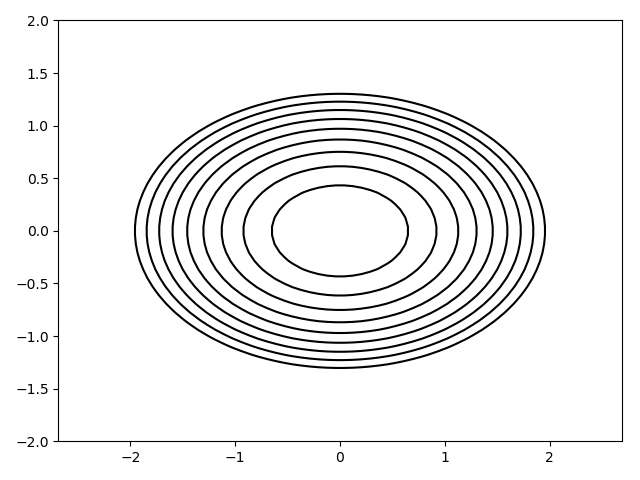
\includegraphics[scale=\myscale,scale=0.5]{figures/fonctions-quadra-1e}
\end{center}

% dessins 3d voir 'fonctions-quadra-1.py' 

\end{exemple}


\begin{exemple}
$$f(x,y) = x^2$$



\begin{itemize}
  \item Les tranches obtenues en coupant selon des plans $y=y_0$ sont des paraboles. Dans l'autre direction, ce sont des droites.
  \item Les lignes de niveau sont des droites.
  \item Le graphe est donc un \defi{cylindre parabolique}.
\end{itemize}

Ci-dessous : (a) la surface, (b) les tranches avec $x$ constant, (c) les tranches avec $y$ constant, (d) les courbes de niveau, (e) les lignes de niveau dans le plan.
\begin{center}
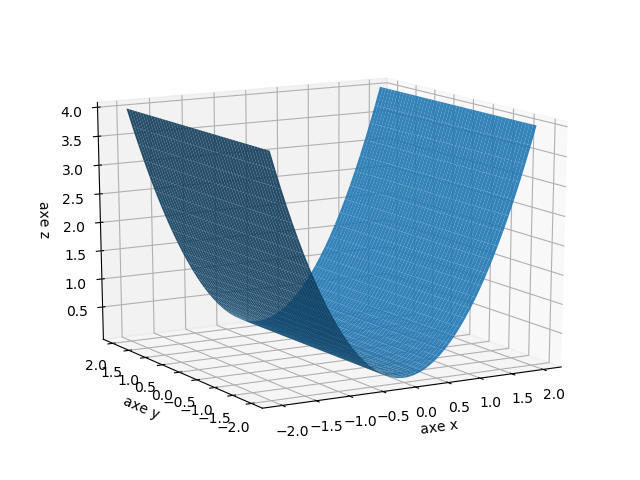
\includegraphics[scale=\myscale,scale=0.5]{figures/fonctions-quadra-2a}
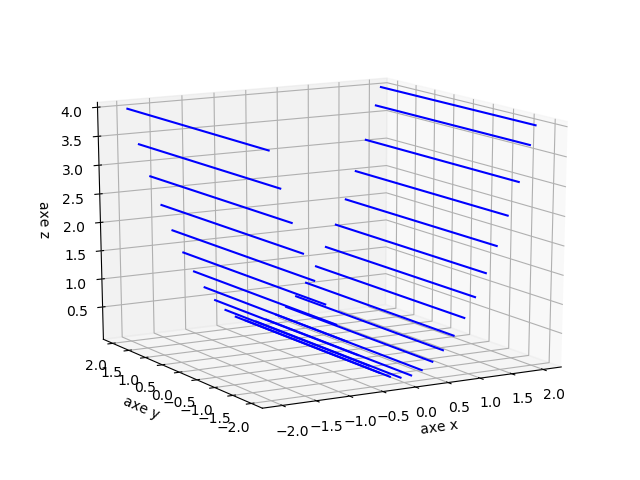
\includegraphics[scale=\myscale,scale=0.5]{figures/fonctions-quadra-2b}
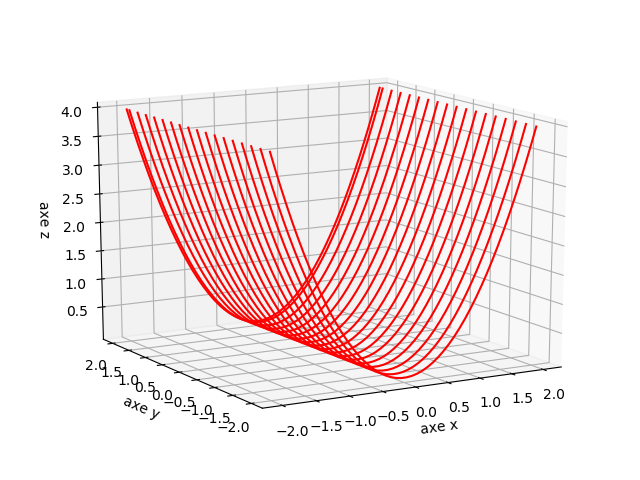
\includegraphics[scale=\myscale,scale=0.5]{figures/fonctions-quadra-2c}
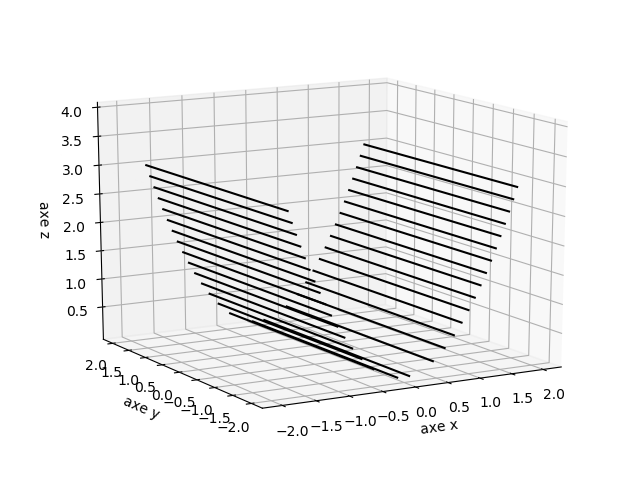
\includegraphics[scale=\myscale,scale=0.5]{figures/fonctions-quadra-2d}
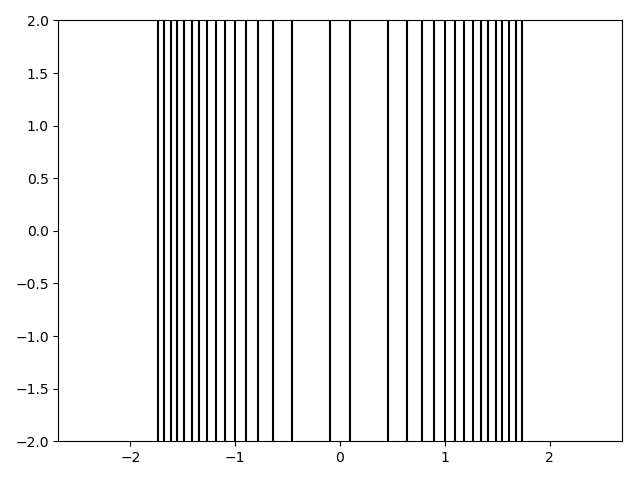
\includegraphics[scale=\myscale,scale=0.5]{figures/fonctions-quadra-2e}
\end{center}

% dessins 3d voir 'fonctions-quadra-2.py' 


\end{exemple}


\begin{exemple}
$$f(x,y) = x^2-y^2$$


\begin{itemize}
  \item Les tranches sont des paraboles, tournées vers le haut ou vers le bas selon la direction de la tranche.
  \item Les lignes de niveau sont des hyperboles.
  \item Le graphe est donc un \defi{paraboloïde hyperbolique} que l'on appelle aussi la \defi{selle de cheval}\index{point-selle}.
  \item Un autre nom pour cette surface est un \defi{col} (en référence à un col en montagne). 
  En effet le point $(0,0,0)$, est le point de passage le moins haut pour passer d'un versant à l'autre de la montagne. 
\end{itemize}

Ci-dessous : (a) la surface, (b) les tranches avec $x$ constant, (c) les tranches avec $y$ constant, (d) les courbes de niveau, (e) les lignes de niveau dans le plan (en pointillé les lignes de niveau négatif).
\begin{center}
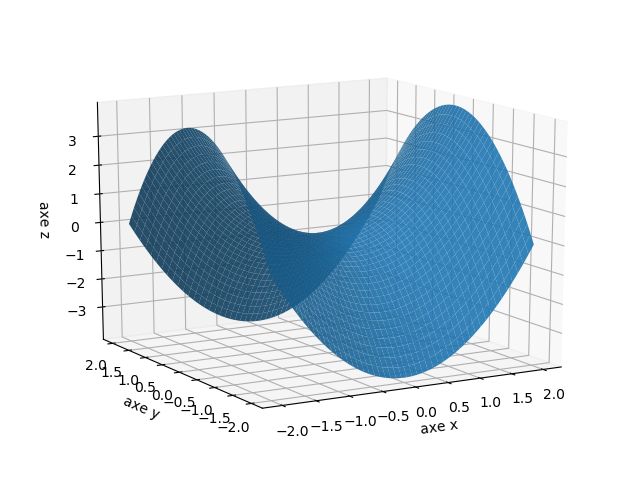
\includegraphics[scale=\myscale,scale=0.5]{figures/fonctions-quadra-3a}
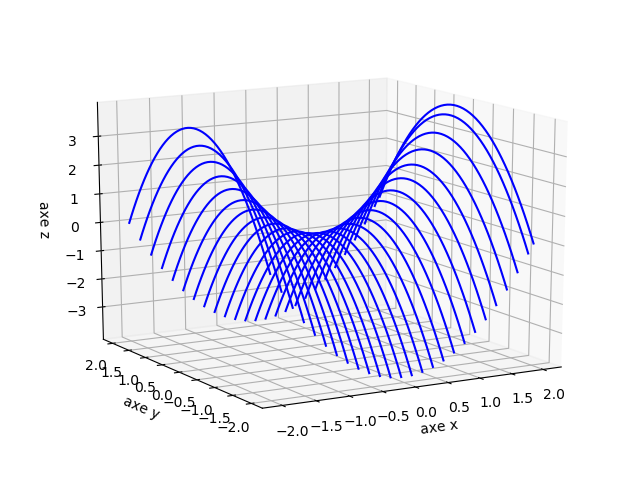
\includegraphics[scale=\myscale,scale=0.5]{figures/fonctions-quadra-3b}
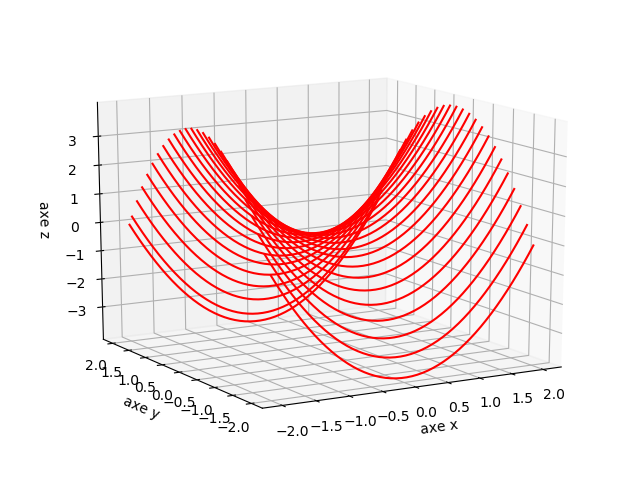
\includegraphics[scale=\myscale,scale=0.5]{figures/fonctions-quadra-3c}
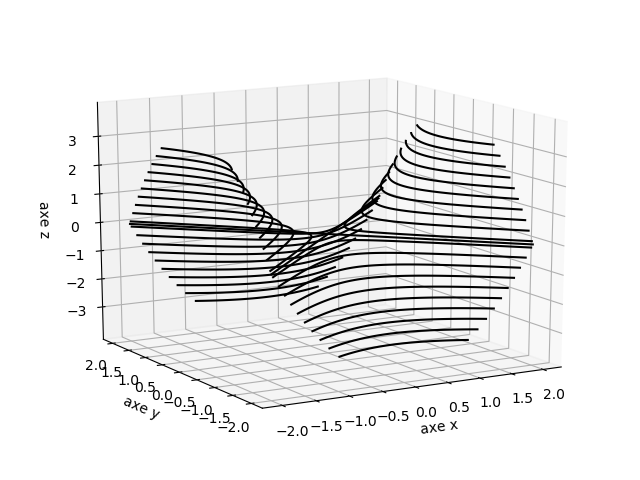
\includegraphics[scale=\myscale,scale=0.5]{figures/fonctions-quadra-3d}
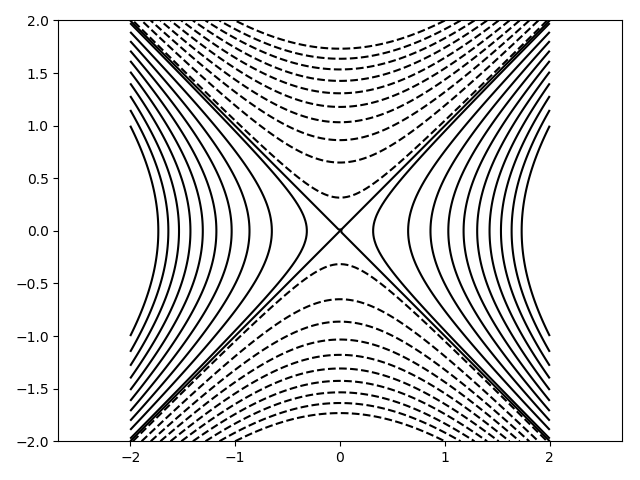
\includegraphics[scale=\myscale,scale=0.5]{figures/fonctions-quadra-3e}
\end{center}

% dessins 3d voir 'fonctions-quadra-3.py' 
\end{exemple}


%--------------------------------------------------------------------
\subsection{Régression linéaire}

\index{regression lineaire@régression linéaire}

\begin{exemple}
On se donne des points du plan, comme ci-dessous. On s'aperçoit qu'ils sont à peu près alignés et on souhaite trouver l'équation d'une droite :
$$y= a x + b$$ 
qui les approche au mieux.


   \myfigure{0.6}{
     \tikzinput{fig-fonctions-10}
   }
   

Formalisons un peu le problème : on se donne $N$ points $A_i(x_i,y_i)$, $i=1,\ldots,N$. Pour une droite $\mathcal{D}$ d'équation $y=ax+b$, la distance entre $A_i$ et la droite $\mathcal{D}$ est donnée par la formule :
$$d(A_i,\mathcal{D}) = \frac{|ax_i-y_i+b|}{\sqrt{1+a^2}}.$$
Pour se débarrasser des valeurs absolues et des racines carrées, on élève au carré et on décide que la droite qui approche au mieux tous les points $A_i$ est la droite qui minimise la fonction 
$$f(a,b) = \sum_{i=1}^{N} d(A_i,\mathcal{D})^2 = 
\frac{1}{1+a^2} \sum_{i=1}^{N}  (ax_i-y_i+b)^2.$$

Pour les $5$ points du dessin initial : $A_1(2,3)$, $A_2(3,5)$, 
 $A_2(4,4)$, $A_4(5,6)$ et $A_5(6,6)$, il s'agit donc de trouver $(a,b)$ qui minimise la fonction 
 $$f(a,b) = \frac{1}{1+a^2} \left( 
 (2a-3+b)^2 + (3a-5+b)^2 + (4a-4+b)^2 + (5a-6+b)^2 + (6a-6+b)^2 \right).$$

 
On trace le graphe de $f$, les lignes de niveau de $f$, et on utilise les techniques à notre disposition pour trouver qu'un minimum global est réalisé en $(a,b) \simeq (0.8,1.6)$, ce qui permet de tracer une droite $y=ax+b$ solution.
 
   \myfigure{0.6}{
     \tikzinput{fig-fonctions-11}
   } 

Lorsque l'on dessine les lignes de niveau, on s'aperçoit que le minimum \couleurnb{(le point bleu) }{}se trouve dans une région plate et allongée. Cela signifie que, bien que le minimum $(a_{\min},b_{\min})$ soit unique, il existe beaucoup de $(a,b)$ tels que $f(a,b)$ soit proche de la valeur minimale $f(a_{\min},b_{\min})$. De plus, ces points $(a,b)$ peuvent être assez éloignés de la solution $(a_{\min},b_{\min})$ (par exemple tous les points de la zone ovale autour du \couleurnb{point bleu}{minimum}). Ce qui signifie que beaucoup de droites très différentes approchent la solution optimale.


\begin{center}
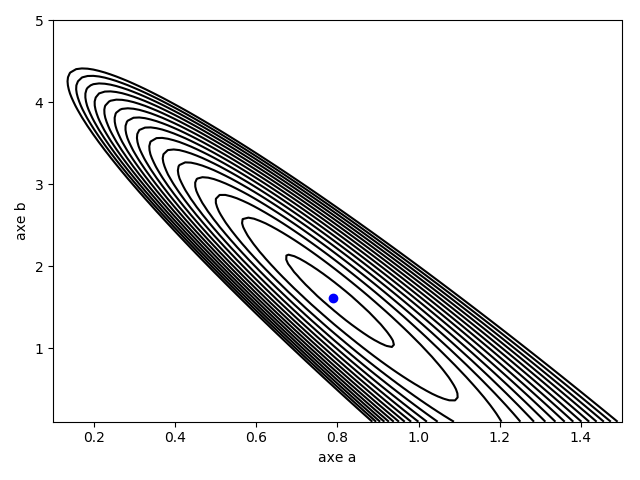
\includegraphics[scale=\myscale,scale=0.7]{figures/fonctions-regression}
\end{center}
% voir 'fonctions-regression-1.py'

\end{exemple}

%%%%%%%%%%%%%%%%%%%%%%%%%%%%%%%%%%%%%%%%%%%%%%%%%%%%%%%%%%%%%%%%%%%%%%
%\section{Ensembles de points du plan et de l'espace}
%
%
%Voici quelques rappels de topologie dans l'espace vectoriel $\Rr^n$. 
%
%\begin{itemize}
%  \item Le \defi{produit scalaire} usuel de $x=(x_1,\ldots ,x_n)$ et $y=(y_1,\ldots ,y_n)$, noté $\langle x \mid y\rangle$, ou bien $x \cdot y$, est défini par
%$$\langle x \mid y\rangle = x_1y_1+\dots +x_ny_n.$$
%
%  \item La \defi{norme euclidienne} sur $\Rr^n$ est la norme associée à ce produit scalaire. Pour $x\in \Rr^n$, la norme euclidienne de $x$, notée $\| x\|$, est définie par
%$$\| x \| = \sqrt{\langle x \mid x\rangle} = \sqrt{x_1^2+\cdots +x_n^2}.$$
%
%  \item La \defi{distance} entre le point $A$ et le point $M=(x_1,\dots ,x_n)$ est $\|M-A\|=\sqrt{(x_1-a_1)^2+\cdots +(x_n-a_n)^2}$.
%  
%  \item La \defi{boule ouverte} de centre $A = (a_1,\ldots ,a_n) \in \Rr^n$ et de rayon $r>0$, notée $B_r(A)$, est l'ensemble suivant :
%$$B_r(A)=\left\{M\in \Rr^n \mid \|M-A\|<r \right\}.$$
%
%
%  \item Soient $U$ une partie de $\Rr^n$ et $A\in U$.
%On dit que $U$ est un \defi{voisinage} de $A$, si $U$ contient une boule ouverte centrée en $A$.
%
%  \item On dit que $U$ est un \defi{ouvert} de $\Rr^n$, si tout pour tout point $A \in U$, $U$ contient une boule ouverte centrée en $A$.
%\end{itemize}
%
%Dans le cas de $\Rr^2$, on note plutôt les coordonnées d'un point par $(x,y)$, alors :
%\begin{itemize}
%  \item $\langle (x,y) \mid (x',y') \rangle = xx'+yy'$
%  \item $\| (x,y) \| = \sqrt{x^2+y^2}$
%  \item $B_r(x_0,y_0) = \left\{ (x,y) \in \Rr^2 \mid (x-x_0)^2+(y-y_0)^2 <r^2 \right\}$ (On parle de \defi{disque} plutôt que de boule.)
%\end{itemize}
%
%De gauche à droite : la distance, un disque ouvert, un ouvert $U$.
%
%\myfigure{1}{
%  \tikzinput{fig-plusvar-12-01}
%  \tikzinput{fig-plusvar-12-02}
%%  \tikzinput{fig-plusvar-12-03}
%} 
%
%
%
%
%%--------------------------------------------------------------------
%\subsection{Ensembles remarquables}
%
%%--------------------------------------------------------------------
%\subsection{Vocabulaire}
% connexe, convexe, segment, polygone, courbe de Jordan


\end{document}
